\chapter{Background and Related Work}

\section{Overview}

In this chapter, the concepts and definitions which are needed to implement the proposed system are identified. In the first section, the tools and concepts borrowed from the relational database management system and in the second section, the concepts in Blockchain technology are introduced. The third section is also dedicated to discuss about the related work and the researches which have been done in this field and compare it with our proposed system.

\section{Temporal Databases}
In this project, we store our historical records in a specific relational database known as the temporal database. A temporal database is any type of database that requires some aspect of time \cite {elmasri2010fundamentalsofdatabase}. Since historical records have a timestamp which indicates the time of a transaction occurrence, in the proposed system, the temporal database is a way to store and manage historical records of the transactions.

%----------------------------------definition Temporal Database-----------------------------------------

\begin{defn}[Temporal database]
	Let $ r_i = \{r_1, r_2, ... , r_n \}$, be $n$ number of tables in the relational database $D$. Denote the attributes of each table as $attr(r_i)$. A temporal table denoted $r_i^T$ is a table with attributes $atr(r_i^T) = \{ (updated, deleted) \in \mathcal{T} \}\cup attr(r_i)$ where $\mathcal{T} = \{t_0,t_1,...,t_n\}$ is the time domain in which transactions on $r_i$ happened. A temporal database denoted $D^T$ is the result of augmenting $D$ by $r_i^T$:

	\begin{center}
		{$D^T = D \cup \{{r_i^T}: r_i \in D \}$}
	\end{center}
\label{dfn:temporal_database}
\end {defn}

The temporal database $D^T$ contains the entire history of the records ever existed in $D$.

\begin{example}
	Given a normal relational table $r_1$ (Table \ref{table:normal_relational_table}) and a temporal table $r_1^T$ (Table \ref{table:temporal_table}), the $attr(r_1) = (id, item, value)$ and $attr(r_1^T)= (id, item, value, updated, deleted)$. The result of query $q_1 = \sigma_{id = 22}(r_1)$ is $\{(22,Pencil,7.50\$)\}$ and the result of same query on the temporal table $q_2 = \sigma_{id = 22}(r_1^T)$ is $\{(22,pencil,8.0\$,2018-03-21,NULL),(22,pencil,7.50\$,2018-03-30,NULL)\}$. Also the query $q_3 = \sigma_{id = 21}(r_1)$ results in $NULL$ however, the same query on the temporal table $q_4 = \sigma_{id = 21}(r_1^T)$ has the history of record with id = 21: $\{(21,ruler,3.25,2018-02-10,NULL),(21,ruler,3.25,NULL,2018-02-20)\}$.
\label{example:temporal_table}
\end{example}

\begin{center}
\begin{table}[t]
	\centering
	\caption{Normal Relational Table $r_1$}
	\label{table:normal_relational_table}
	\begin{tabular}{p{4cm}p{4cm}p{4cm}}
		\hline
		id & item      & value  \\ \hline
		22 & Pencil    & 7.50\$ \\
		23 & Notebook & 12.0\$   \\ \hline
	\end{tabular}
\end{table}

\begin{table}[t]
	\centering
	\caption{Temporal Table $r_1^T$}
	\label{table:temporal_table}
	\begin{tabular}{p{1cm}p{2cm}p{3cm}p{3cm}p{2cm}}
		\hline
		id & item      & value  & updated  & deleted\\ \hline
		21 & Ruler    & 3.25\$  & 2018-02-10  &  - \\  
		21 & Ruler    & 3.25\$  & -  &  2018-02-20 \\
		22 & Pencil    & 8.0\$  & 2018-03-21  &  - \\
		22 & Pencil    & 7.50\$  & 2018-03-30  &  -\\
		23 & Notebook & 12.0\$  & 2018-04-01 & - \\ \hline
	\end{tabular}
\end{table} 
\end{center}

%---------------------------------- End of Definition Temporal Database -----------------
%---------------------------------- Defintion Time Domain -------------------------------
\begin{defn}[Time domain]
	The time domain $\mathcal{T}$ consists of discrete timestamps $t_0,t_1,...,t_n$ in which transactions on tables $r_i \in D$ happened. the range of time domain is: $\mathcal{T} = [t_0, \infty)$ where $t_0$ is the timestamp in which the first record added to the table $r_i$.
\label{dfn:time_domain}
\end{defn}

The time domain of a temporal table $r_i^T \in D^T $ is calculated by:

\begin{center}
	$\mathcal{T} = r_i^T[updated] \cup r_i^T[deleted]$
\end{center}
For example in the temporal table $r_1^T$ (Table 2.2), the time domain is:
$\mathcal{T} = [2018-02-10,2018-04-01]$.
%---------------------------------- End of Definition Time Domain -----------------------
%---------------------------------- Defintion Timestamps --------------------------------
\begin{defn}[Timestamps]
	A timestamp $t_i \in \mathcal{T}$ is a particular position in the time domain, in which particular transaction(s) happened. For example in the temporal table $r_1^T$ (Table 2.2), ``2018-03-30'' is a timestamp in which the record with ``id = 22'' updated.
\label{dfn:timestamp}
\end{defn}
%---------------------------------- End of Definition Timestamps ------------------------
%---------------------------------- Defintion Timeline ----------------------------------
\begin{defn}[Timeline]
	Let $u_i(t_j)$ be the total transactions on the tables $r_i \in D$ at timestamps $t_j \in \mathcal{T}$, where $i,j=\{0,1,...,n\}$. The $u_i(t_j)$ could be represented as an ordered set points on a vector. This vector is called a timeline for the transactions happened on $r_i \in D$.
\label{dfn:timeline}
\end{defn}
Figure \ref{fig:timeline} illustrates the concept of timeline.

\begin{figure}
	\centering
	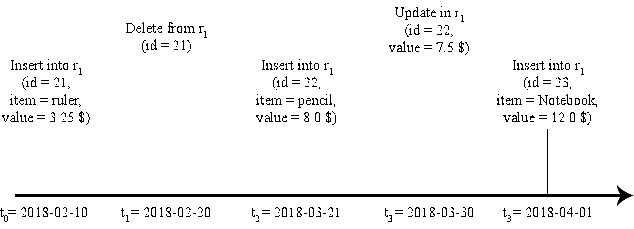
\includegraphics[width=\textwidth]{figs/timeline.pdf}
	\caption{Timeline.}
	\label{fig:timeline}
\end{figure}

%---------------------------------- End of Definition Timeline --------------------------
%---------------------------------- Defintion snapshot ----------------------------------
\begin{defn}[Snapshot and snapshot-queries] 
	Given a temporal table $r^T \in D^T$ and a timestamp $t \in \mathcal{T}$, we denote $s(t)$ to be the table instance that obtained by calculating the $\{max(r^T[m])|t : m\in r)\}-r^T[deleted]$ for $\mathcal{T}\leq t$. Note that $s(t) \in D^T$ but not necessarily $s(t) \in D$. A snapshot is a materialized version of $D(t) = \{s_1(t),s_2(t),...,s_n(t)\}$. A snapshot-query is an arbitrary relational query on $D(t)$.
\label{dfn:snapshot}
\end{defn}

We can construct the snapshots using simple windowing functions (as in supported by PostgreSQL \cite{momjian2001postgresql}).

    \vspace{1em}
\begin{center}

{\small
	\begin{tabular}{|l|} \hline
		$\mathrm{snapshot}(r, t)$ = \\
		\verb|| \textsc{With} $T$ \textsc{as} ( \\
		\verb| | \textsc{select} id, $\{\mathrm{last\_value}(x) \mathrm{\ as\ } x:
		x\in attr(r)\}$ \textsc{over} $W$ \\
		\verb| | \textsc{from} $r^T$ \\
		\verb| | \textsc{where} updates $\leq t$ \\
		\verb| | \textsc{window} $W$ \textsc{as} 
		\textsc{partition by} id \textsc{order by} updates\\
		\verb|| ) \\
		\verb|| \textsc{select} id, $\{x: x\in attr(r)\}$ \textsc{from} $T$ \\
		\verb|| \textsc{where not} $T.$deleted \\ \hline
	\end{tabular}
}
\end{center}

The query $\mathrm{snapshot}(r, t)$ computes the snapshot of $r$ at timestamp $t$ by applying the latest update of each tuple up to timestamp $t$, while removing tuples that have been deleted.

%---------------------------------- End of Definition snapshot --------------------------


\section{Blockchain}
In a big picture, Blockchain technology is a distributed trusted public ledger that the stored data in it is immutable and it is open to anyone to inspect \cite{OECD2016Science}. Although today there are a numerous number of applications that are using Blockchain \cite{dhillon2017blockchain},  ‌Blockchain is mostly known for its application in cryptocurrencies such as Bitcoin \cite{nakamoto2008bitcoin}. As a matter of fact, Blockchain is the secret why cryptocurrencies are secure, work in a decentralized network, do not need any central verification system and although all transactions are transparent, the users in the system are anonymous \cite{halaburda2016beyond}.
While there are many functionalities within a Blockchain system, such as user anonymity, being public and no need for a central verification system, in this project, for the sake of confidentiality and transparency, not all functionalities within the Blockchain is employed. To understand how Blockchain has been utilized in the proposed system, there are some definitions that need to be discussed beforehand.

%---------------------------------- Begin of Definition cryptography --------------------------
\begin{defn}[Cryptography]
	Cryptography is a way of secure communication between parties in a network while adversaries might also be present. Using Cryptography, messages sent or received are encrypted so that the adversaries cannot read the normal form of the message. This communication is established through various steps such as cryptographic key assignment, encryption, and decryption of messages or digitally signing a message and verifying the digital signatures \cite{stallings2017cryptography}.
\label{dfn:cryptography}
\end{defn}
%---------------------------------- End of Definition cryptography ----------------------------
%----------------------------- Begin of Definition cryptographic keys -------------------------
\begin{defn}[Cryptographic Keys]
	Let $u$ be the authenticated user who is using database $D$. By the creation of the profile of $u$ in the system, a set of strings $<K_{priv}, K_{pub}> \in \mathbf{N}^+$ is generated and assigned to the user where $K_{pub}$ is the public key that is accessible to everyone on the system, and $K_{priv}$ is the private key that is known only to $u$. These keys are used to encrypt/decrypt messages which are transmitted between the users\cite{stallings2017cryptography}.
\label{dfn:cryptographic_keys}
\end{defn}
%----------------------------- End of Definition cryptographic keys -------------------------
%----------------------------- Begin of Definition Assymetric Encryption --------------------
\begin{defn}[Assymetric Encryption]
	Let $E$ be the encryption algorithm, $D$ be the decryption algorithm, $m$ be the message which needs to be encrypted and $c$ be the encrypted message. Given the cryptographic keys $<K_{pub}, K_{priv}>$, An encryption technique is said to be asymmetric if:
	\begin{center}
		$c = E(K_{pub},m)$ and  $m = D(K_{priv},c)$
	\end{center}
	or
	\begin{center}
		$c = E(K_{priv},m)$ and  $m = D(K_{pub},c)$
	\end{center}
	Therefore:
	\begin{center}
		$D(E(m,K_{pub}),K_{priv}) = m$ 
	\end{center}
	and
	\begin{center}
		$D(E(m,K_{priv}),K_{pub}) = m$
	\end{center}
\label{dfn:assymetric_encryption}
\end{defn}

Note that, if $K_{pub}$ is known, and $E(K_{pub},m)$ is also known, in asymmetric encryption method, it is impossible to get $m$ without $K_{priv}$ \cite{stallings2017cryptography}.
Figure \ref{fig:AssymmetricEncryption} shows the basic steps to send and receive messages between two parties in a secure way by utilizing asymmetric encryption technique. In this scenario, the sender has access to the recipient's public key only. The sender encrypts the document which is to be transferred by using the recipients public key. In asymmetric technique, the only way to decrypt the document is to use the recipient's private key which the is only known to the recipient. This is a powerful technique to ensure that the adversaries cannot read the document in the middle of the connection.

\begin{figure}
	\centering
	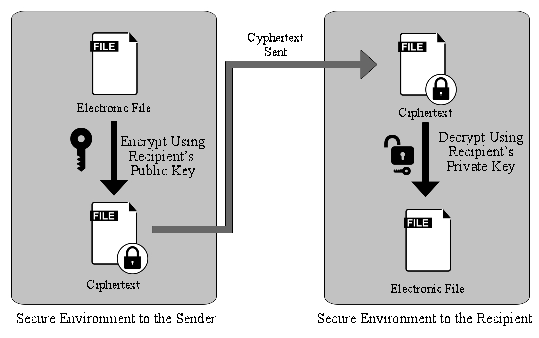
\includegraphics[width=\textwidth]{figs/asymmetricEncryption.pdf}
	\caption{Asymmetric Encryption Technique.}
	\label{fig:AssymmetricEncryption}
\end{figure}
%----------------------------- End of Definition Assymetric Encryption --------------------
%----------------------------- Begin of Definition Hash function --------------------------
\begin{defn}[Hash function]
	Assume $m \in \mathcal{A}$ to be the message with an arbitrary size chosen from domain $\mathcal{A}$. $hash(m)\rightarrow sketch$ is a function that maps the $m$ of any size from domain $\mathcal{A}$ to a fixed size string (normally 256 bits) in a smaller domain $\mathcal{B}$ \cite{aumasson2014thehash}.
\label{dfn:hash_function}
\end{defn}
%----------------------------- End of Definition Hash function ----------------------------
%----------------------------- Begin of Definition Digital Signature ----------------------
\begin{defn} [Digital signature]
	Let $m$ be the document which needs to be digitally signed and transferred. Denote $h$ as the hash function, $E$ as the encryption algorithm and $D$ as decryption algorithm. In order to digitally sign a document and verify a signature, the following steps are taken:
	\begin{itemize}
		\item \textbf{Step 1.} $H_r = h(m)$
		\item \textbf{Step 2.} $S = E(H_r,K_{priv})$
		\item \textbf{Step 3.} $m$ and $S$ are sent
	\end{itemize}
\label{dfn:digital_signature}
\end{defn}

A digital signature is used to ensure that the digitally transferred data has not been altered while transferring. Also, it verifies whether or not the transferred data was submitted by a recognized source \cite{katz2010digital}.\\

\begin{defn}[digital signature verification]
	In order to verify a digital signature the following steps are taken:
	\begin{itemize}
		\item \textbf{Step 1.} $m$ and $S$ are received
		\item \textbf{Step 2.} $H_t = h(m)$ is calculated
		\item \textbf{Step 3.} $H_r = D(S,K_{priv})$ is obtained
		\item \textbf{Step 4.} $m$ is valid if $H_t = H_r$ and invalid otherwise.
	\end{itemize}
\label{dfn:signature_verification}
\end{defn}

Figure \ref{fig:DigitalSignature} depicts the steps that needs to be taken to digitally sign a document and verifying a digital signature.\\
\begin{figure}
	\centering
	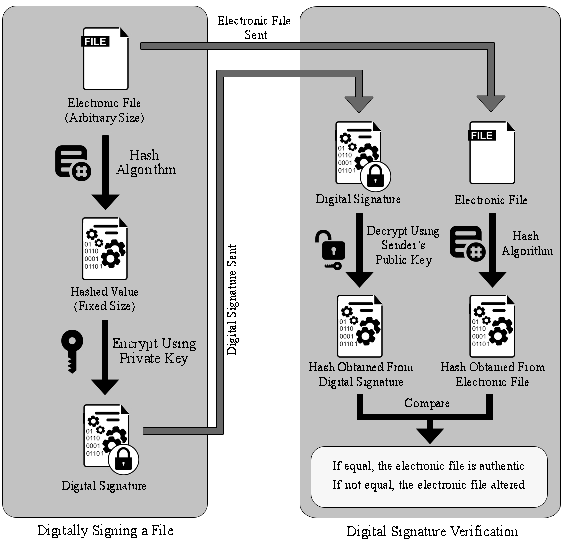
\includegraphics[width=\textwidth]{figs/digital_signature.pdf}
	\caption{Digital Signature Creation and Verification.}
	\label{fig:DigitalSignature}
\end{figure}
%----------------------------- End of Definition Digital Signature ----------------------------
%------------------------------------- Defintion Blockchain -----------------------------------
\begin{defn}[Blockchain] 
	Let $rec_i$ be the records stored in $r_i^T$. We denote $Sign$ as $S_r(attr(r_i^T$ for $rec_i))$ which is digital signature of attributes of $rec_i$. We can create a blockchain of historical records by storing the signature of the previous record as an attribute of the current record.
\end{defn}
The idea of the Blockchain has been depicted in figure \ref{fig:Blockchain}.
\begin{figure}
	\centering
	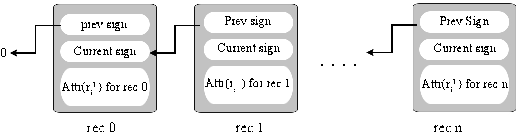
\includegraphics[width=\textwidth]{figs/blockchain.pdf}
	\caption{Idea of the Blockchain for the proposed system.}
	\label{fig:Blockchain}
\end{figure}

\section {Related Work}
There has been a wide range of studies on ensuring the trustworthiness of records in a database from different perspectives. These studies range from establishing trust between nodes in a real-time distributed systems \cite{khayat2017trust} to secret sharing schemes in cloud databases \cite{dutta2013privacy} and utilizing logfiles for forensic purposes \cite{sinha2014continuous}. In this project, the assumption is that the preventive models are not able to stop the adversaries from manipulating the data of a relational database system, therefore a tamper-evident log table has been offered to evaluate whether or not the data has been altered. 

Database audit logs contain valuable information such as any insertions, deletions, and modifications of the records performed in a database along with the timestamp of the performed tasks. The United States Department of Defense in its “Trusted Computer System Evaluation Criteria” document and under requirement 4 pointed out the importance of auditing the transactions in a computer system in a secure and efficient manner \cite{USDoD1985}. In this document also protecting the audit logs from modification or destruction has been stressed out. ”ISO/IEC 27001” standard published by International Organization for Standardization and International Electrotechnical Commission \cite{ISOIEC27001}, “Guide to Computer Security Log Management” standard published by United States National Institute of Standard and Technology \cite{NIST2006}, eHealth Ontario's HER standard \cite{ehealth3542}, European Commission Information System Security Policy C(2006) 3602 \cite{EC2006} and the University of British Columbia's information Security Standard {\#}17 \cite{UBC2014} are a few of many other international or domestic regulations that have suggested guidelines to secure computer systems by using historical records such as audit logs.

Analyzing audit logs for forensic purposes has been the topic of research by many scientists, however, since the trustworthiness of the results from log table analysis has a direct relationship with the authenticity of the records of the log file, a lot of studies have been carried out to make log tables tamper-proof. Haber {\it et al.}\cite{haber1991how} proposed a basic methodology by utilizing timestamping and hash chains in order to make unmodifiable historical records for digital documents. Peha in \cite{peha1999electronic} offered a method to detect log tampering by one way hashing and employing multiple trusted notaries to keep track of all transactions. The author argued that if any notary decided to falsify the transaction, the attempt is discovered by other notaries. Snodgrass {\it et al.} \cite{snodgrass2004Tamper} also offered one-way hashing mechanism and employed trusted notaries, however in order to enhance the security of the method offered by Peha, they offered to hash the records with a timestamp of previous transaction modification. Schneier {\it et al.}\cite{schneier1998cryptoraphic} offered a cryptographic-based mechanism to create hash chains and make the log files nearly impossible for the attacker to alter. The validity of the transactions was also done by trusted third-parties who have the cryptographic keys.

However the aforementioned researches might have promising results to protect the historical records from being compromised by an outsider, but they have one thing in common which is the role of an insider to carry out malicious attacks is forgotten. Also hiring third-party software/hardware may bring up a lot of privacy concerns. Therefore, unlike the mentioned works, not only our proposed system does not require a third-party notary to attest the authenticity but also it does not put trust on any user of the system.

The role of privileged users in acting maliciously in a database has been discussed by many researchers \cite{crosby2009tamper-evident} \cite{wagner2018detect}. Liu {\it et al.} offered a network-based auditing mechanism which also keeps track of privileged users' activity and performs audit analysis through event correlation. Wagner {\it et al.} \cite{wanger2017carving} proposed a mechanism to detect database file tampering by looking for inconsistencies in the database's storage. The authors argued that the databases follow patterns in storage which even the privileged users have no access to. Therefore, if a record is deleted maliciously in the log file, the inconsistency in the storage is evident for a period of time. Unlike mentioned proposed methods, our system uses inherent to RDBMS tools and does not require a network-level-auditing mechanism or having access to the server's storages, therefore it could be easily implemented on remote servers and relational databases on cloud storages. Also, our proposed system not only discovers maliciously deletion of the records but also identifies any malicious modification without any time constraints.

For the sake of gathering verifiable pieces of evidence, in our proposed system, any changes to the database regardless of the users' access privileges need to be tracked. This action could be done by utilizing inherent to DBMS tools. Fabbri {\it et al.} \cite{fabbri2013select} extensively talked about SELECT triggers which are inherent RDBMS functions, required database specifications and efficient implementation techniques for data auditing. Hauger {\it et al.}\cite{hauger2014information} also discussed the use of triggers in the database for forensic purposes. Triggers are supported by RDBMS which makes them a good candidate to be used in our proposed system however, it is naive to assume that a simple trigger solely is secure enough to be used for forensic purposes. Therefore we propose to use the Blockchain technology to make immutable chains of transactions that are captured by database triggers.

The first attempt to use chained hashes for securing data from tampering is known to be done by Haber {\it et al.} \cite{haber1991how} where the authors proposed a methodology to securely timestamp the digital files and create digital signatures and hash chains. This work was then improved by Schneier {\it et al.} \cite{schneier1998cryptoraphic} \cite{schneier1999minimizing} \cite{schneier1999secure} by offering to exchange secret codes with a trusted third party who is able to verify the authenticity of the chain. They offered a method to change the shared secret as the new transaction occurs, therefore since the attackers do not have the previous secret codes, it is impossible for them to alter any records which were previously added. Our proposed method is similar to the mentioned works in this aspect that our historical records are chained together using the digital signatures, however, we use asymmetric encryption without the need of a third-party to attest the authenticity of the transactions.